\documentclass{scrartcl}
\usepackage{multicol}
\usepackage{epigraph}
\usepackage{url}
\usepackage{listings}
\usepackage{graphicx}
\usepackage{color}
\usepackage[parfill]{parskip}
\usepackage{titlesec}
\usepackage{geometry}
\usepackage{todonotes}
\usepackage{hyperref}
\usepackage{booktabs}
\usepackage{longtable}
\usepackage{array}
\usepackage{textcomp}

\lstset{
breaklines=true,
breakautoindent=true,
postbreak=\space,
tabsize=2,
basicstyle=\ttfamily\footnotesize,
showspaces=false,
showstringspaces=false,
extendedchars=true,
}

\newcommand{\horizontalrule}[1]{\rule{\linewidth}{#1}}
\def\changemargin#1#2{\list{}{\rightmargin#2\leftmargin#1}\item[]}
\let\endchangemargin=\endlist

\newcounter{savepage}

\setlength{\LTleft}{0pt}

\title{\horizontalrule{1pt}\\[0.5cm]Large-scale drive-by download detection: visit$^n$. process. analyse. report.}
\subtitle{Master in System and Network Engineering \\[0.5cm] \horizontalrule{1pt} }
\author{}
\date{}

\begin{document}
\pagenumbering{gobble}
\newgeometry{top=4cm,bottom=1cm}

\centerline{
\includegraphics[width=10cm]{Images/UvA-logo-english}}

\begin{center}
\horizontalrule{1pt}\\[0.5cm]
\usekomafont{title}{\huge Large-scale drive-by download detection: \\[0.2cm] visit$^n$. process. analyse. report.}
\\[0.1cm]
\usekomafont{subtitle}{Master in System and Network Engineering} \\[0.5cm]
\horizontalrule{1pt} 
\end{center}

\vspace{7cm}

\begin{center}

\Large
Students:\\[0.5cm]

\begin{minipage}{0.4\textwidth}
\begin{flushleft} \Large
Adriaan Dens\\\texttt{adriaan.dens@os3.nl}
\end{flushleft}
\end{minipage}%
\begin{minipage}{0.4\textwidth}
\begin{flushright} \Large
Martijn Bogaard\\\texttt{martijn.bogaard@os3.nl}
\end{flushright}
\end{minipage}\\[1.6cm]

\Large
Supervisors:\\[0.5cm]

\begin{minipage}{0.4\textwidth}
\begin{flushleft} \Large
Jop van der Lelie\\\texttt{jop.vanderlelie@ncsc.nl}
\end{flushleft}
\end{minipage}%
\begin{minipage}{0.4\textwidth}
\begin{flushright} \Large
Wouter Katz\\\texttt{wouter.katz@ncsc.nl}
\end{flushright}
\end{minipage}\\[1.6cm]

{\Large \today}
\end{center}

\clearpage
\restoregeometry

\section*{Abstract}

Current malware analysis systems do not allow for concurrently visiting multiple websites. In this paper we present an algorithm which solves this problem by hooking into the APIs that a browser uses. The data received from the API hooking is added into a graph (without loosing the URL context), after which analysis of malware can be done. Additionally, a proof of concept has been developed which implements this algorithm. Results show a significant performance gain compared to current systems.

\clearpage

\tableofcontents

\clearpage

\pagenumbering{arabic}
\newgeometry{bottom=5cm}

\section{Introduction}
In the digital world of today, malware is still a massive and growing problem. While it was used to annoy users and system administrators in the early days, nowadays it is used for extortion, cyber espionage and surveillance by criminal groups and rivalling governments. One of the main causes of getting infected with malware is a drive-by download while visiting a normal day-to-day website because, for example, the website got hacked and infected. 

In many cases \cite{proofpoint,foxittelegraaf,foxityahoo} however, it was not the actual website but one of the advertisement networks that was compromised and which subsequently started serving malicious code hidden in innocentl-looking advertisement code. This is also called malvertising \cite{Li2012}.

National CERT organisations are interested in an early detection of such threats. While automated systems to scan websites already exist, like Cuckoo\footnote{http://cuckoosandbox.org} and Anubis\footnote{http://anubis.iseclab.org}, one of the main downsides is the time needed to analyse multiple websites.

The goal of this research project is to develop an algorithm that makes it possible to examine multiple websites for the existence of malware using the same computer system and at the same time, increasing the speed at which detection can occur. The effectiveness of this algorithm will be proved by implementing it in a proof of concept.

\subsection{Research Question}

In cooperation with the Dutch National Cyber Security Center (NCSC-NL), our research project focuses on the question:

\textit{How can we concurrently visit multiple URLs and still be able to determine which URL was responsible for malicious activities?}

To answer the research question, multiple sub-questions have been formulated:

\begin{itemize}
\item Which techniques are used by web browsers to make concurrently visiting multiple URLs possible?
\item Which APIs are used by web browsers to make HTTP requests and retrieve webpages?
\item How can an HTTP request be correlated to its source URL without the modification of the used web browser?
\item Which additional information sources (from the client or its environment), besides what was used to correlate HTTP requests, can be used to make the tracking of malware to its source URL easier?
%What extra information from the client's (running) machine can be used to augment the information gained from network traffic to make the tracking of malware to its source URL easier?
\end{itemize}

\pagebreak
\restoregeometry

% \subsection{Motivation?}

\subsection{Related work}

The growing threat of malware resulted in many research projects in the last few years. The detection and analysis of malware has been researched from several different angles \cite{auto_malware,Chang2013} and resulted in many proposed static and dynamic analysis techniques.

In 2013, Le \textit{et al.} \cite{Le2013} presented a framework that describes the common stages and characteristics of a drive-by download attack. They described four stages from placing the malicious content on a webpage to the execution of the malicious activity.

In 2011, a paper from Canali \textit{et al.} \cite{Canali2011} was released about the problematic performance of dynamic analysis and with a solution proposed in the form of ``Prophiler''. Prophiler is a filter that deploys static analysis techniques and that is able to reduce the load by more than 85\% compared to dynamic analysis. This result was realised without a significant change in the amount of false negatives.

In the same year Rajab \textit{et al.} \cite{Rajab11trendsin} gave an overview of the trends regarding web malware detection and how the malware tries to circumvent detection. This research focused on the advantages and disadvantages of four techniques: Virtual Machine honeypots, Browser Emulation honeypots, Classification based on Domain Reputation and Anti-Virus Engines.

A different approach was taken by Rossow \textit{et al.} \cite{Rossow2011}; Cortjens and El-Yassem \cite{Cortjens2012}; Kinkhorst and Van Kleij \cite{Kinkhorst2009}. During multiple research projects they focused on the ability to detect and identify malware on the network layer.

The usage of graphs to detect malware has been proposed before. Park and Reeves proposed \cite{Park2011} the usage of graphs of system calls to detect the similarities and differences in behaviour between the variations of a malware family. By focusing on the common subgraph, new variants can be detected and categorized without prior knowledge of their existence. A recent paper  from W\"{u}chner \textit{et al.} \cite{Wuchner2014} described the usage of generating graphs from API calls for a heuristic-based malware detection system.

The predecessor of NCSC-NL (GOVCERT.NL), together with NASK/CERT Polska, started in 2007 with the development of their own system, the Honeyspider network \cite{honeyspider}, for the dynamic analysis of websites. This system crawled the biggest and most important websites of the Netherlands on a daily base. The downside of this system is that it requires a lot of maintenance and therefore it started to become outdated.

\iffalse
\subsection{Scope}

\todo{Zelfstandiger maken}

In this research project is an an algorithm created that allows multiple URLs to be opened at the same time while still being able to track all further interaction, such as unexpected HTTP requests and other malicious activity, and link them to the original request/URL. To prove that the algorithm is something feasible, a proof of concept of the algorithm has been implemented on top of the Cuckoo Sandbox.

The goal during this research project was to make the algorithm fully platform agnostic, however, several technical challenges prevented this. For this reason we limited our self to Windows 7 with version 8 of the Internet Explorer browser and have we the identified issues described.

The detection and identification of malicious behaviour was not part of this project. For our PoC we sticked to the detection of a well-known older and still to be determined malware family which existence is easy to detect on the system. 

\subsection{Ethical issues}

% Zinnen herschrijven die naar de toekomst verwijzen.
Our research contains no major ethical issues as it does not include working with personally identifiable information. Malware, if any, will be run in a controlled virtual environment. After every testrun the virtual machine will be automatically destroyed.

\fi


\clearpage

\section{Theory}
For a better insight into the project, it is necessary to introduce certain theoretical concepts first. In the next chapter this theory will be used to base the approach on for the design and development of the algorithm and choices regarding the proof of concept.

\subsection{Drive-by downloads}

Browsing the internet with an unpatched system, for example because the patch is not installed or there is simply no solution available, can be dangerous. All software contains mistakes and such mistakes are patched almost on a daily basis. Part of those mistakes can be (ab)used to get control over a computer system and be used to run malicious software without the user noticing.

If a website uses such mistake to take control over the web browser and download malicious software to the system, this is called a drive-by download. Figure \ref{fig:dbdownload} shows the steps involved from visiting a website until the moment the system is infected with malware.

By compromising the web browser and injecting malicious code, the malware gets full control over the infected process, running with the same privileges as the web browser on the host system. Depending on the system configuration this either means that full system access is available or that additional steps are required to escalate the privileges to the intended level.


\begin{figure}[h]
    \centering
    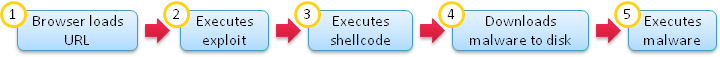
\includegraphics[width=12cm]{Images/drive-by-download.png}
    \caption{The anatomy of a drive-by download malware infection. \cite{http://blog.armorize.com/2011/04/newest-adobe-flash-0-day-used-in-new.html (modified)}}
    \label{fig:dbdownload}
\end{figure}

\subsubsection{Behavior}

What happens after a malware infection depends on the malware used and goals of the attacker. In many cases the malware will download further malicious components and nestle itself in the operating system so it can be restarted after a reboot of the operating system and is able to restore itself after an attempt to remove it.

To do this, the malware has to modify files, registry values \todo{is Windows specific} and perform network operations. While theoretically malware could directly communicate with the kernel for this, most malware behaves like a normal application and uses the installed, or with the operating system provided, libraries. The usage of such libraries can be detected when the access to them is monitored.

\subsection{API analysis}

In the early days, libraries were primarily used by an application by statically linking to it. This means that the library becomes part of the application and it is no longer possible to determine which part of the application was originally part of the used libraries.

For performance and maintainability, dynamic linking was invented. The application describes which libraries it needs and the linker of the operating system will glue the applications and its dependent libraries together in the memory space of the application. 

Because the linker has to know all exported functions and where in the library it can find such function, a symbol table is part of every dynamic library. The same information can be used to hook into an provided function during runtime or to trick the linker to load a replacement of a certain function because the modified version has a higher priority.

This is called API hooking\cite{} and it is a very useful technique to monitor the behavior of applications. The original function is replaced by a substitute. This substitute function calls, for example, the original function and logs the performed operation or \todo{change sentence} is a custom replacement of the original function.

The technical implementation of API hooking is highly complex and platform specific. Many different techniques\cite{http://jbremer.org/x86-api-hooking-demystified/} of hooking are possible as well. If the start of the application can be controlled, the linker search path can be extended to include the replacement library. Alternatively, the import section of the application can be modified. When the application is already loaded or modification of the application or system is unwanted, the function to hook can be overwritten in memory with a replacement or jump to a different location in memory. However, this will prevent the ability to execute the original function unless the overwritten bytes are carefully preserved and reconstructed somewhere else.

In this project API hooking will be used to reverse engineer the internal workings and API usage of web browsers and to log the behavior of malware for later analysis.

\subsection{Web browser architecture}
% Target: 4-6 blz

\todo{Meer bronnen?}

Modern web browsers are complex applications consisting of many components which have to work together. To develop a generic algorithm, it is crucial to have an in-depth understanding of the inner workings of a web browser. This project focuses on Internet Explorer, Mozilla Firefox, Chromium and Apple Safari. Those four browsers combined have a marketshare of more than 90\%\footnote{http://gs.statcounter.com/\#desktop-browser-ww-monthly-201412-201412-bar} \footnote{http://www.netmarketshare.com/browser-market-share.aspx?qprid=1\&qpcustomb=0}.

All modern web browsers allow the usage of multiple tabs in a single window. The underlying implementations of those tabs differ greatly. Internet Explorer and Safari use only libraries provided by the operating system while Firefox and Chromium decided to use their own libraries. Some browsers decided to use multiple processes and sometimes even a new process for every single tab.

\textbf{Internet Explorer} supports tabs since version 7 and version 8 was improved with the ability to run tabs in their own process (see figure \ref{fig:ie8proc}). This feature is called ``loosely-coupled IE''\cite{IE8LCIE}. Every process runs independent from the other processes and runs with its own network stack and instances of content plugins like Flash or Silverlight.

Starting each tab in its own process comes with an inevitable overhead of using more memory and a slower startup. For this reason a process in Internet Explorer can host multiple tabs. The amount of tabs in a single process and the maximum number of processes is determined by the configuration. For backwards compatibility, Internet Explorer also provides the option to disable the usage of multiple processes and host all tabs in a single browser process.

\label{sec:brie}
The network stack used in Internet Explorer is provided by the Windows operating system and is called WinINet\cite{wininet}. This library provides high-level access to functions that allow HTTP and FTP requests and utility functions for caching, proxies and security. After initiating and configuring the request, WinINet will perform the necessary steps to execute the request. WinINet depends on the Winsock library \cite{winsock} to setup the required network connections and Schannel \cite{schannel} is used to provide transparent support for SSL/TLS connections.

\begin{figure}
    \centering
    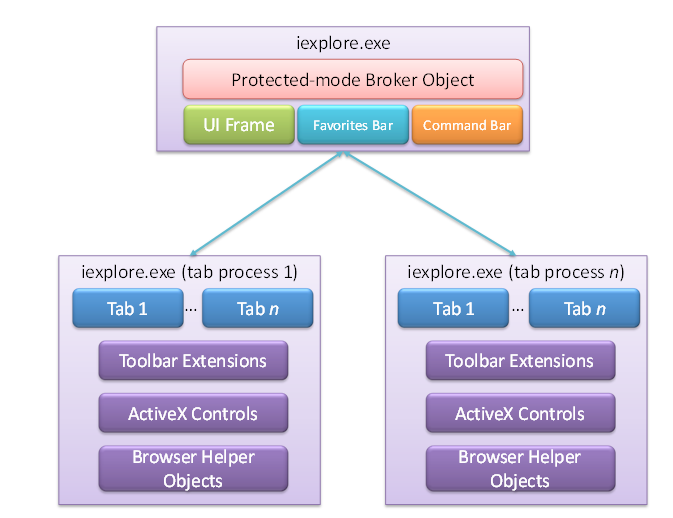
\includegraphics[width=9cm]{Images/IE8_process_model.png}
    \caption{The Internet Explorer process model starting from version 8. \cite{IE8LCIEP}}
    \label{fig:ie8proc}
\end{figure}

\textbf{Firefox} uses only a single process for web content and only runs plugins from a different process. A long-term project to change that is called Electrolysis\footnote{https://wiki.mozilla.org/Electrolysis} and has been developed since 2009. In the new architecture, the entire rendering moved to a dedicated and sandboxed ``content'' process and the main process is used to host the user interface and serves as a proxy between the outside world and the content process. A longer-term goal is to spread the rendering of multiple tabs over more than one content process so when a content process crashes not all tabs are affected.

To be platform independent, Firefox does not directly interface with the provided libraries of the operating system. Instead a platform-neutral API called ``NSPR'' (Netscape Portable Runtime, \cite{nspr}) is used. Together with the Network Security Services (NSS, \cite{nss}) library that provides the functionality to create SSL/TLS connections, both are used by the high-level network library called Necko. Necko provides the interface to perform HTTP and other protocol requests without revealing the underlying protocol, transport level or platform specific implementation details and is thus comparable to WinINet.

\textbf{Chromium} is the open-source version of the Google Chrome browser and it is except for a couple of proprietary components identical to Chrome. The big innovation of Chrome \cite{ChromeMPA} was to use multiple processes instead of a single process. Besides its own process for every tab, it also has the plugins and audio subsystem in their respective processes. The subprocesses run in a sandbox with limited privileges and use the main process to communicate with the outside world.

\begin{figure}[h]
    \centering
    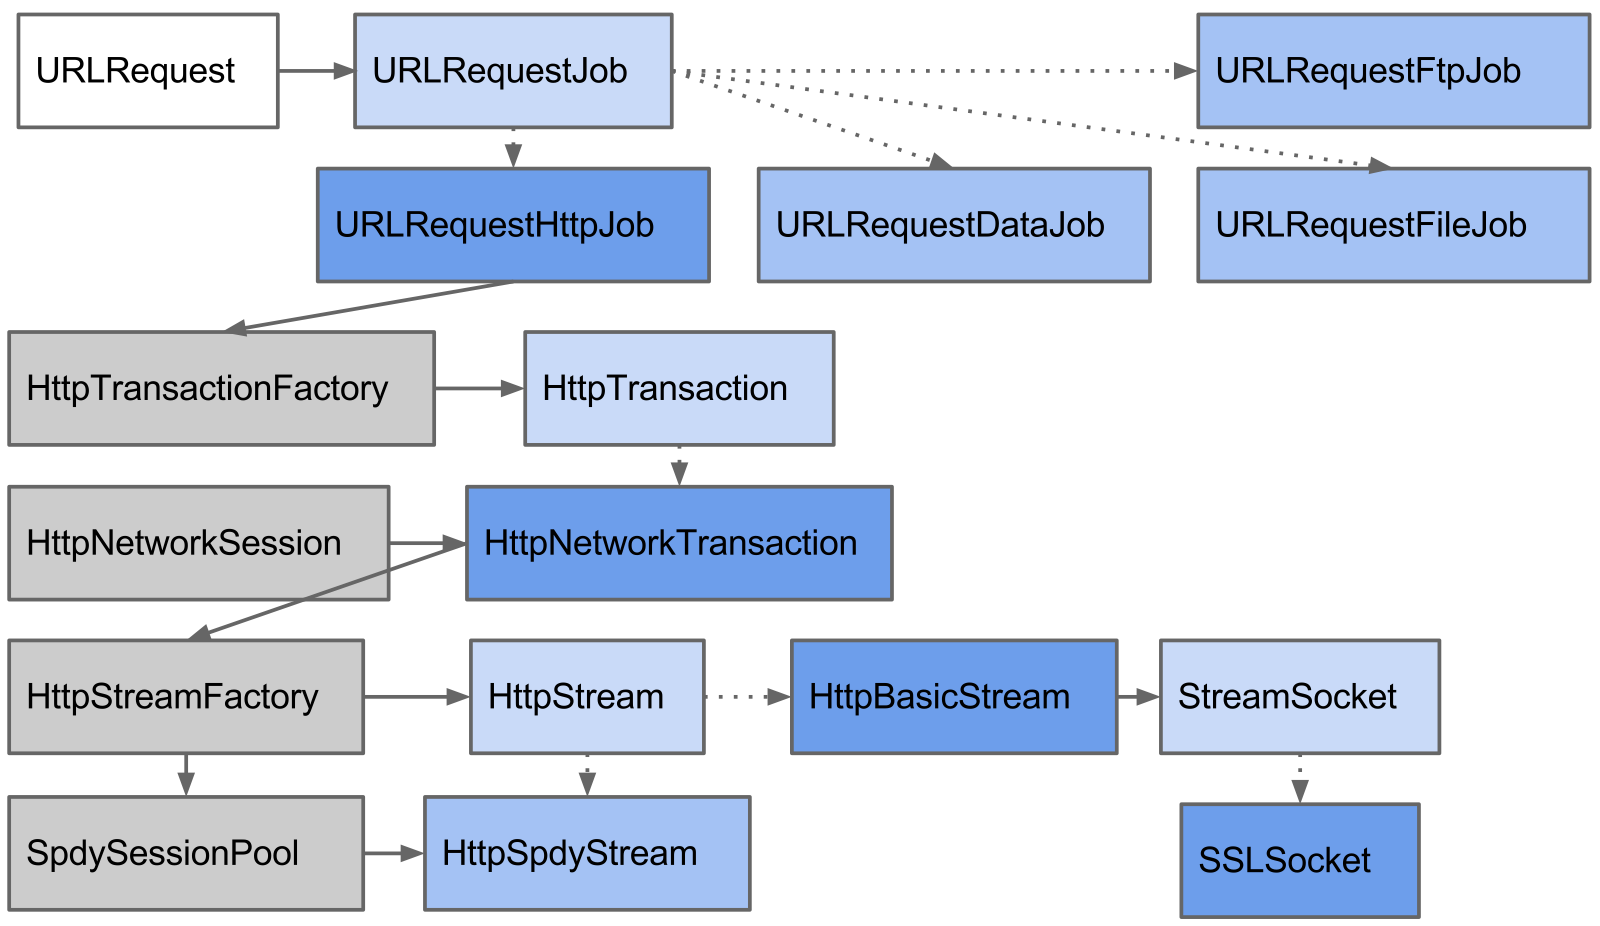
\includegraphics[width=9cm]{Images/Chrome_network.png}
    \caption{A high-level overview of the components involved in requesting an URL in Chromium. Platform specific details related to sockets are hidden in StreamSocket and the usage of SSL/TLS is made transparent by using the interface-compatible SSLSocket instead of StreamSocket. \cite{ChromeNetwork}}
    \label{fig:chrome_network}
\end{figure}

The library used by Chromium for network access is custom developed and tightly integrated in the engine. It provides similarly functionality as Necko and WinINet using a high-level interface (see figure \ref{fig:chrome_network}) but also it contains low-level interfaces that interface directly with the operating system's socket API. To provide transparent SSL/TLS support, the same library as Firefox is used, NSS.

\textbf{Safari} is the last browser that was examined in this project. Since 2011\footnote{https://lists.webkit.org/pipermail/webkit-help/2011-July/002298.html} support for using multiple processes has been added. Safari is closed-source but build on top of many open-source components like JavaScriptCore and WebKit.

Safari uses a dedicated process for every tab until a certain limit is reached. Once this limit is reached, multiple tabs are hosted in a single process. The network operations for the main and tab processes is concentrated in a dedicated process. Only this process will retrieve the webpages and use IPC mechanics to deliver the result to the correct process. 

CFNetwork is the library that is used by Safari for its network access. This library is one of the core frameworks of the OS X operating system and available for all applications. It provides interfaces for all relevant web related protocols. A unified interface called NSUrl, similarily to other browsers, is also available. However, because of the closed-source nature of Safari it is not possible without an extensive reverse engineering effort to determine if it is used instead of directly using the provided APIs of the CFNetwork library.

\iffalse

Which techniques are used by browsers to make concurrently visiting multiple
URLs possible?
	- Tabs of course
		- As a process
		- As multiple threads under the browser process

How can we link an HTTP request to its source URL without the modification of the used web browser?
we need extra information, see vraag 4
network is niet genoeg blablabla

How do web browsers make HTTP requests and retrieve webpages? Which Operating System level APIs are used?
	- Safari: CFNetwork and NSURLConnection(Loader) and IPC
		1 hoofdprocess: Safari
		1 process per tab: Safari Web Content
		1 process voor networking: Safari Networking
		Network stack of OS X.
	- Internet Explorer: C API calls naar Windows libraries
		Process per tab: is configureerbaar in settings/registry, je kan ook meerdere tabs in 1 process hebben
		Network stack of Windows
	- Firefox: C++ Library calls
		Single Process (+ 1 process voor flash)
		Own network stack Necko (nss3 voor trafiek te encrypten)
		\url{https://developer.mozilla.org/en-US/Firefox/Releases/3.5/Updating_extensions#Getting_a_load_context_from_a_request}
		http://stackoverflow.com/questions/10719606/is-it-possible-to-know-the-target-domwindow-for-an-httprequest
	- Chrome: IPC 
		1 hoofdprocess: Google Chrome die networking doet
		1 process per tab. (Altijd 13 threads?)
		1 process voor Flash.
		1 process voor Audio. (4 threads)
		Own network stack (nss3 voor trafiek te encrypten)
		http://www.chromium.org/developers/design-documents/network-stack

What extra information from the client's (running) machine can be used to augment the information gained from network trac to make the tracking of malware to its source URL easier?  
	- The Thread ID or Process ID van tabs, PDF reader, Java applet, ...
	- Handle bij IE
	- File descriptors
	- Process tree
	- Voordeel van op machine network traffic te intercepten is dat we rommel van andere applicaties niet zien, maar enkel het trafiek van de browser en de gespawnde subprocessen ervan.
	- 
\fi



\clearpage

% \newgeometry{bottom=0.1cm}
\section{Approach and Methods}
In this section, we discuss our approach for the large-scale detection of drive-by downloads and how we want to implement it in a proof of concept. But we start with investigating how to correlate different HTTP requests that logically belong together.

\subsection{Correlating HTTP requests}
\label{sigh}

The challenge faced when multiple websites have to be loaded at the same time, is to know which HTTP request corresponds to which website. Many webpages consist of dozens of resources that have to be loaded. The loading of some resources can even be delayed until after certain predefined events. In some libraries, the requesting of a web resource consists of several independent steps.

A solution would be to modify the web browser in such a way that it exposes this information with an easy to use interface. While this would solve the problem, regular maintenance would be required to keep this system working as the browser executable has to be changed for every release.

Another solution could be to log all the network traffic and analyse it. While this information is always available, it would require complex protocol and content parsers to reconstruct the original network streams and extract useful information from it. Additionally, an encrypted connection would require a proxy that uses on-the-fly creation of certificates. Even then it would be trivial to circumvent this system as scripting languages and browser plug-ins could be used to dynamically request resources.

% \thispagestyle{empty}
% \restoregeometry

A better solution would be to correlate an HTTP request to its originating webpage by observing the behaviour and environment of the web browser. By hooking and logging the API calls that are made by the web browser, the full process and thread context of every call is available or can be reconstructed from earlier calls (as can be seen in figure \ref{fig:wininet}). As all modern web browsers use high-level network libraries, this is the ideal place to monitor. When combined with other interesting APIs, a full insight in the behaviour of the web browser is available and detecting malicious behaviour is a matter of writing the correct behavioural analysers.
\begin{figure}[h]
    \centering
    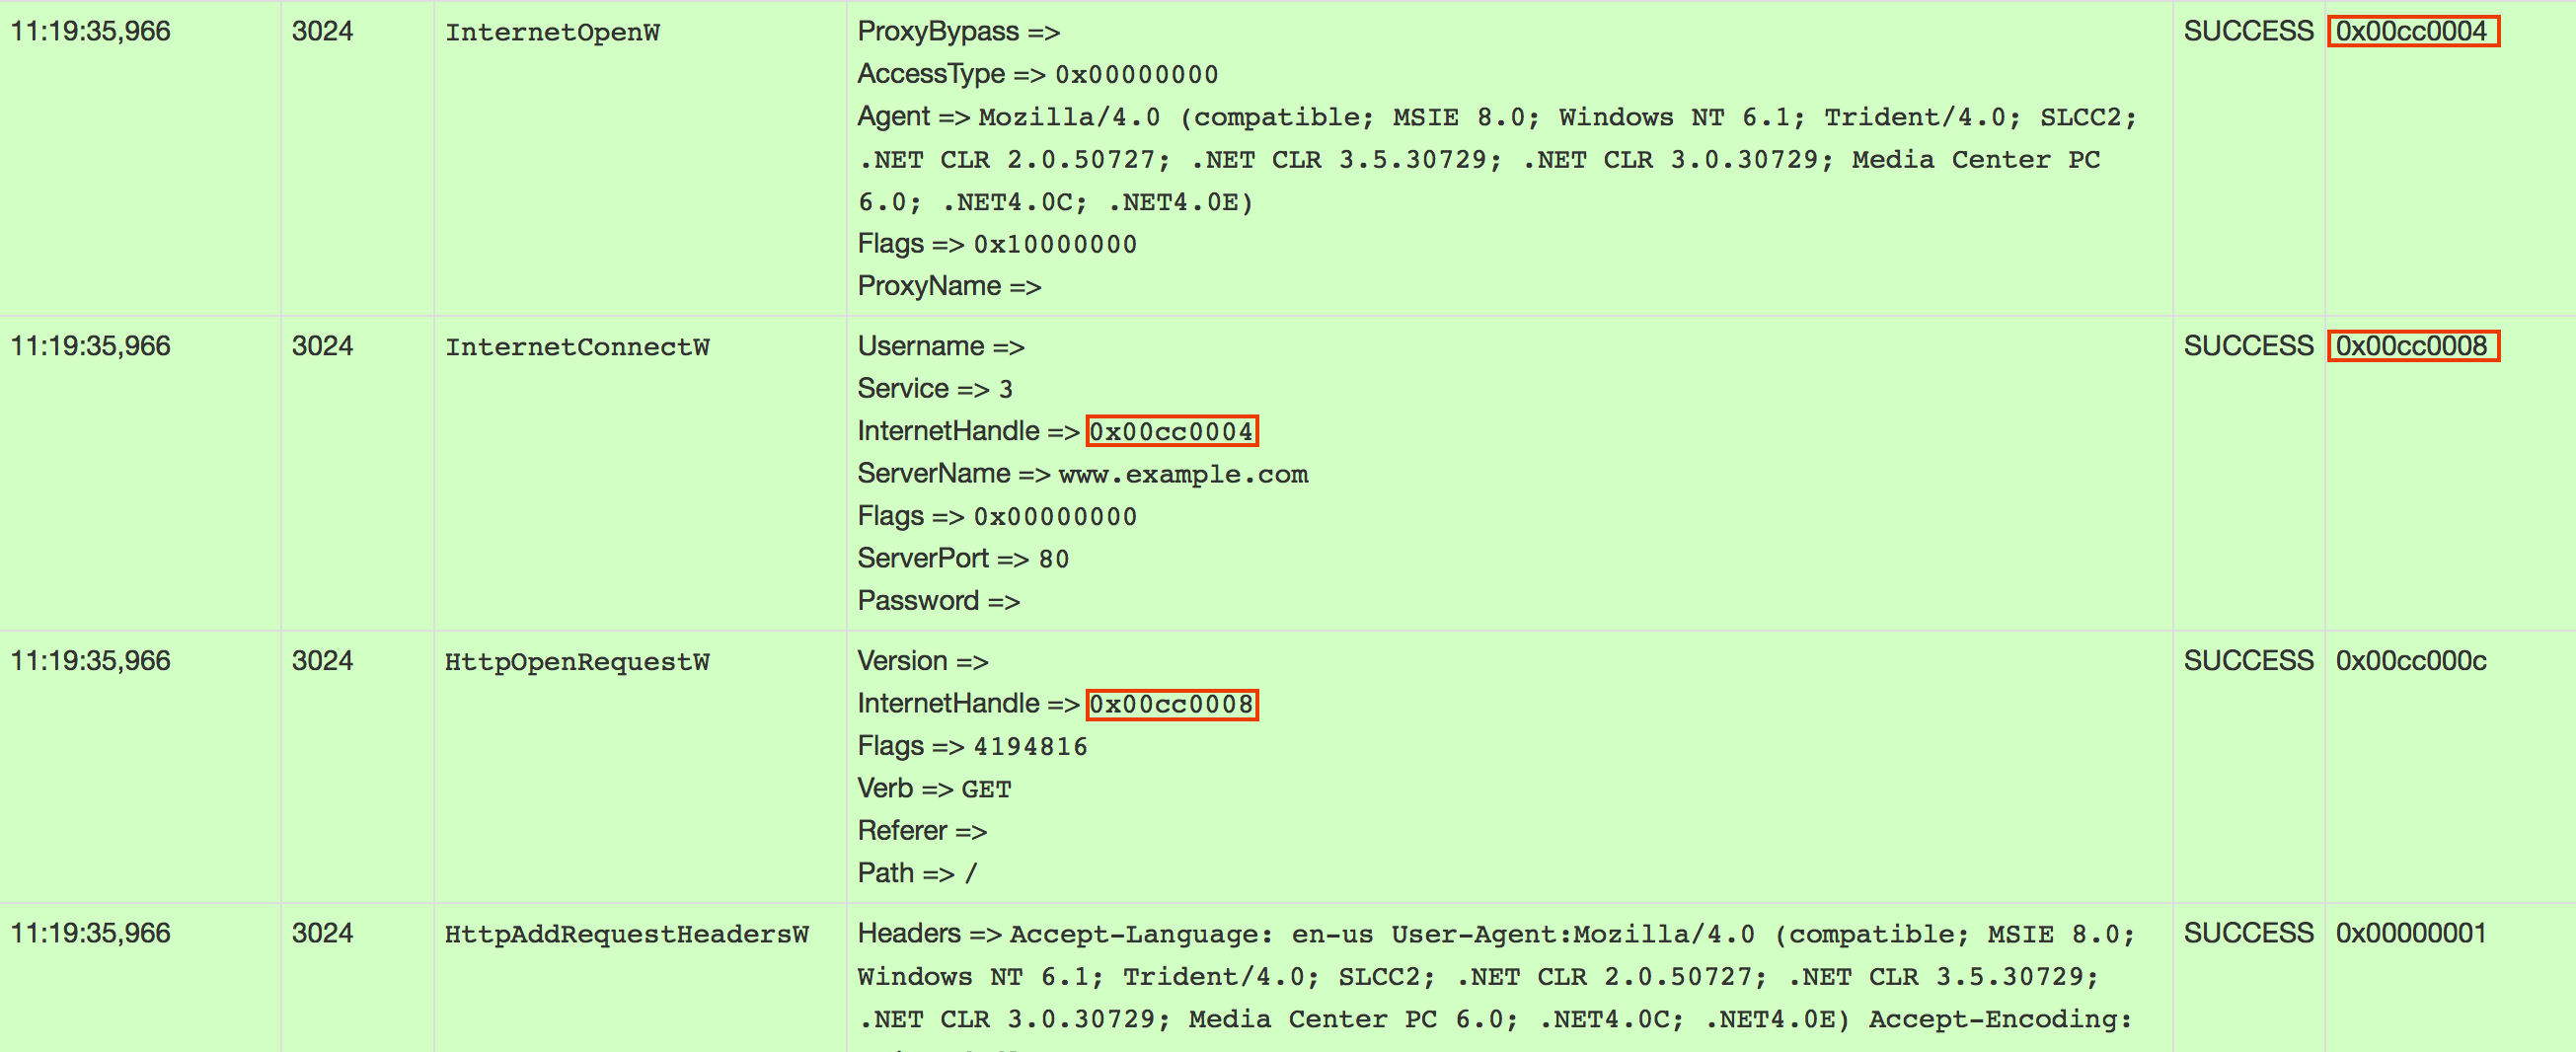
\includegraphics[width=14.7cm]{Images/wininet.png}
    \caption{Example of the API calls involved when the WinINet library is used to load a URL. The red rectangles show the handles that can be used to identify the API calls that belong to a single request.}
    \label{fig:wininet}
\end{figure}

An alternative for API hooking would be to write a custom operating system driver and monitor the syscalls. While this would still give most of the information API hooking would give and much harder to detect by the malware, it is much harder to implement and the information gained from intercepting the API calls to the high-level network libraries would not be available.

\subsection{Algorithm}
\begin{figure}[h]
    \centering
    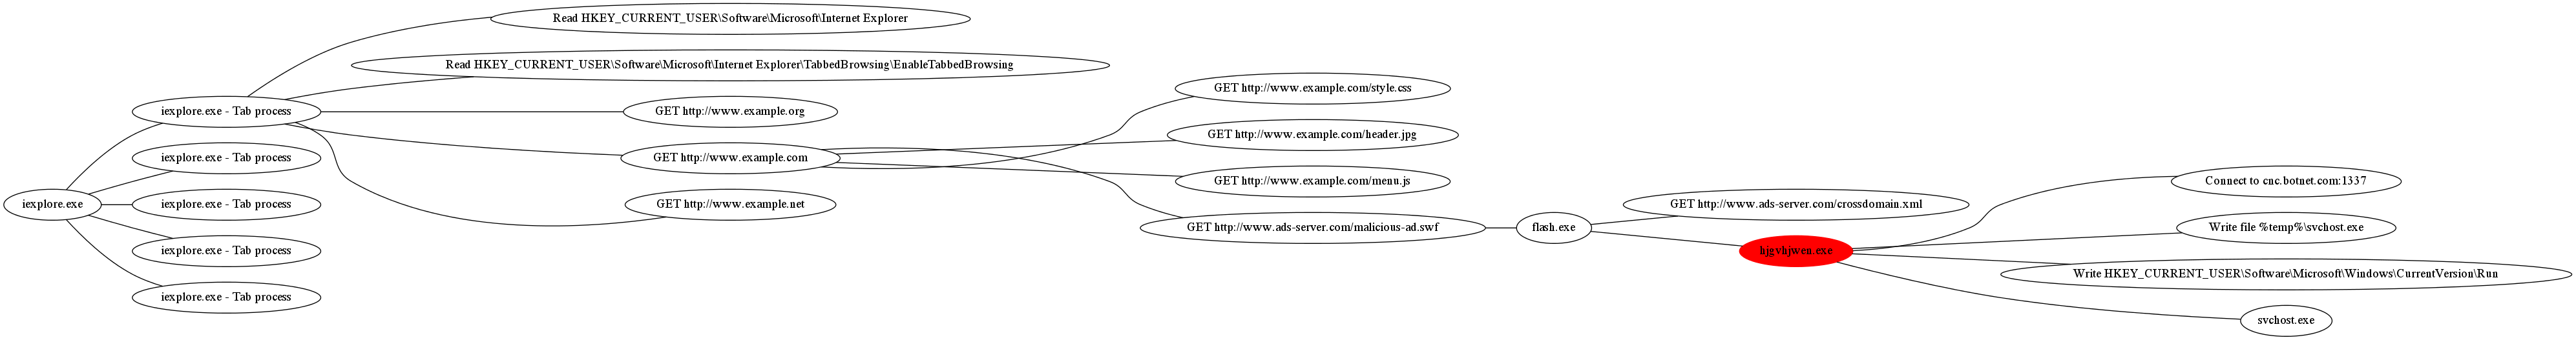
\includegraphics[width=17cm]{Images/alg_tree.png}
    \caption{An example of the graph}
    \label{fig:alg_tree}
\end{figure}

\subsubsection{Design considerations}

\subsubsection{Generic algorithm}

- Disconnected DAGs

1) Hooker schrijven voor elke browser die trafiek tussen Netwerk en Browser of in de browser zelf monitort en doorgeeft aan Cuckoo
2) DAG opstellen door de extra informatie te gebruiken in report.json
3) DAG interpreteren, nodes met enkel uitgaande edges zijn de beginnende URL
4) Kijken of er iets raar gebeurt in elk eiland
5) Reporting

\subsubsection{Platform-specific challenges}

Unix heeft geen handles zoals Windows maar meer files
	- FD's eigenlijk

\subsubsection{Alternative approaches}

- pcap / mitm
- tijd based
- aangepaste headers

\subsection{Proof of concept}
\epigraph{You're the chosen one, Cuckoo.}{Adriaan}

\textbf{TOEKOMSTIGE TIJD}

For the Proof of Concept (PoC), Cuckoo \cite{cuckoo} will be used. Cuckoo is a malware analysis system that runs malware in a virtual environment, tracks its behavior and reports these results to the user.\\

Cuckoo was choosen because it already implements a great deal of the prerequisites of the algorithm, discussed in \todo{add ref}. Cuckoo, through Cuckoomon \cite{cuckoomon}, provides a series of hooks which monitors calls between the browser and the operating system. This allows us to monitor the extra information from section \ref{algo2}. 

These hooks, conveniently, also monitor the network calls made by the browser. Although only Internet Explorer is supported by Cuckoo, due to the scope of the project, this is not a problem.

\subsubsection{Prerequisites and changes}

Internet Explorer uses Windows' ``Secure Channel'' or ``Schannel'' \cite{schannel} to encrypt HTTP requests and decrypt HTTP responses. This will allow us to monitor traffic on the operating system level without any need for a proxy to decrypt the traffic.

As already explained, Cuckoo uses Cuckoomon, which uses hooks to monitor calls, to keep track of the browser activity. Besides adding a few new hooks and deleting a few irrelevant hooks for drive-by downloads, nothing major has to be changed to Cuckoomon.\todo{Uitleggen welke hooks precies?}

The current development version, \texttt{1.2-dev},  only accepts one URL at a time. To allow for concurrently visiting multiple websites in one sandbox environment, Cuckoo has to be extended.

\subsubsection{The Setup}

To test the algorithm, we will use the adapted Cuckoo with Virtualbox as the sandbox environment. As the virtual machine's operating system, we will use Windows 7 as this is still the operating system which is most targeted by malware. As the browser, we will use Internet Explorer 8 to actually allow the malware to successfully perform the drive-by download.

The virtual machine will be provisioned with the Top 20 of visited websites in the Netherlands, according to Alexa \cite{http://www.alexa.com/topsites/countries/NL}, and with current malware floating on the internet.\todo{Mss toch niet zeggen?}

The structure of the graph will be tree-like, as suggested in \todo{ref naar algo}. Figure \ref{fig:alg_tree}.

Figure \ref{fig:alg_tree} also shows a website with a drive-by download. In the top left, one can see process spawns (red vertices) in an unusual place.\todo{beter uitleggen}

\begin{figure}[h]
    \centering
    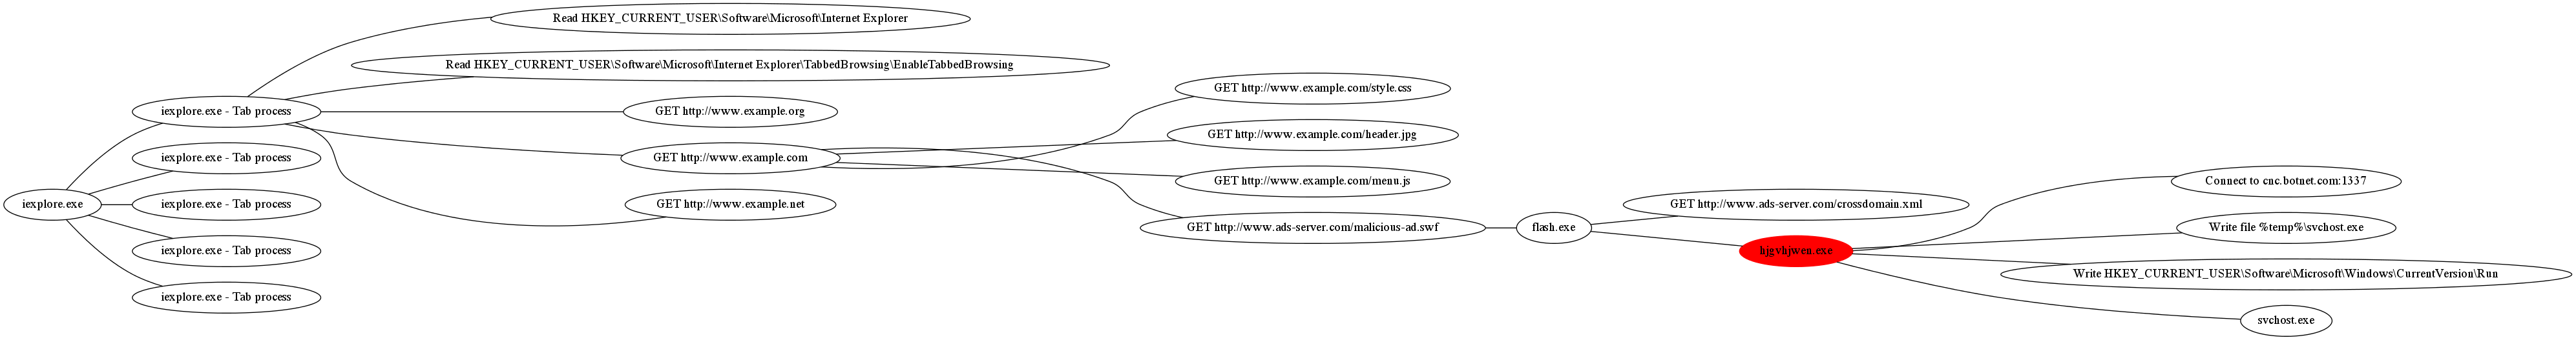
\includegraphics[width=17cm]{Images/alg_tree.png}
    \caption{An example of the graph}
    \label{fig:graph}
\end{figure}




\clearpage

\section{Results}
\todo{Rewrite chapter introduction}

\subsection{Implementing the algorithm}

\subsubsection{Step 1: Visit}

To support the parallel visiting of URLs in one virtual machine, we had to extend Cuckoo. Support for this was added pretty quickly using tabs, but this left us with a problem to detect when a new URL was feeded to a tab\todo{See problems below}. To solve this problem, every URL is now opened in its own window.

\subsubsection{Step 2: Process}
\begin{description}
\item[on\_process\_new] sfdsfdf
\item[on\_process\_finished] sfdsfdf
\item[on\_http\_request] sfdsfdf
\item[on\_file\_write] sfdsfdf
\item[on\_file\_delete] sfdsfdf
\item[on\_registry\_set] sfdsfdf
\item[on\_registry\_delete] sfdsfdf
\item[on\_shell\_execute] sfdsfdf
\item[on\_socket\_connect] sfdsfdf
\item[on\_anomaly\_detected] sfdsfdf
\end{description}
\subsubsection{Step 3: Analyze}

To implement the analysis phase of the algorithm, a simple analyzer was written that detects process spawns below browsing contexts. Listing \todo{reffie} shows pseudo code of the analyzer.

\begin{lstlisting}
function deep_process_spawn_analyzer(graph)
    foreach vertex in graph
        if vertex.type == "process_spawned"
            if check_depth_in_graph(vertex, 0) > 1
                print "Malicious activity"
            endif
        endif
    endforeach
endfunction

function check_depth_in_graph(vertex, current_depth)
    parents = get_parents_of_vertex(vertex)
    # Actually we need only one parent
    if length_array(parents) > 0
        return check_depth_in_graph(parents[0], current_depth++)
    else
        # No more parents, we're at the root node
        return current_depth
    endif
endfunction
\end{lstlisting}

\subsubsection{Problems}
\label{99problems}
\epigraph{I've got 99 problems but Cuckoo ain't one.}{Adriaan}

\begin{itemize}
\item Out of order openen en sluiten van handles 
\item Paralellizatie problemen
\item BSON file loggen naar de host
\item Weten wanneer een nieuwe URL wordt geopend
\begin{itemize}
\item Geen TypedURLs met COM
\item COM (CrossZoneCompare, blocking Navigate met deadlock tot gevolg, )
\end{itemize}
\item Opsplitsen / linken van de data in 1 process over meerdere requests
\item Missende data door te kleine buffers en niet geimplementeerde apis in cuckoomon
\end{itemize}

\subsection{Step 4: Report}
\todo{Betere analyzer reporting in output script...}
\begin{lstlisting}
$ python cuckoo.py &
$ python utils/mass-analyse.py -g -t 22
Warning: Task with ID 22 is not yet completed; Waiting...
INFO:root:Parse log....
Analyzer 'Subprocess_from_tab': The URL 'http://malware-site.com' 
spawns a process called 'errfix.exe'.
\end{lstlisting}

\subsection{Running the PoC}
\newgeometry{left=3cm,top=0.1cm,bottom=0.1cm}
 \todo{Explain the colors of the vertices}
\begin{figure}[h]
    \centering
    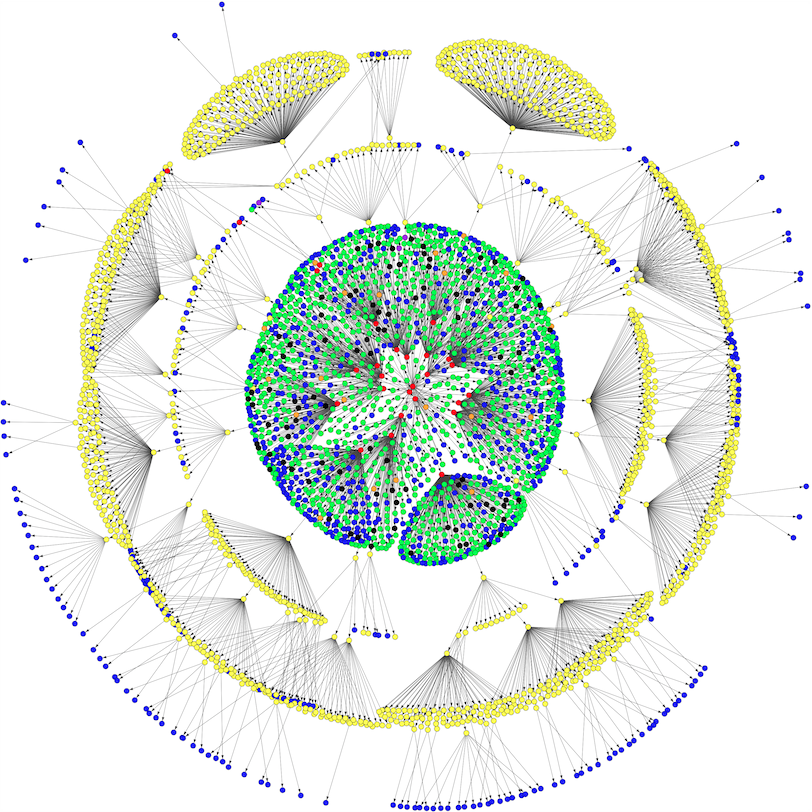
\includegraphics[width=17cm]{Images/graph2.png}
    \caption{An example of the graph}
    \label{fig:graph}
\end{figure}
\subsubsection{Step 6}
\begin{figure}[h]
    \centering
    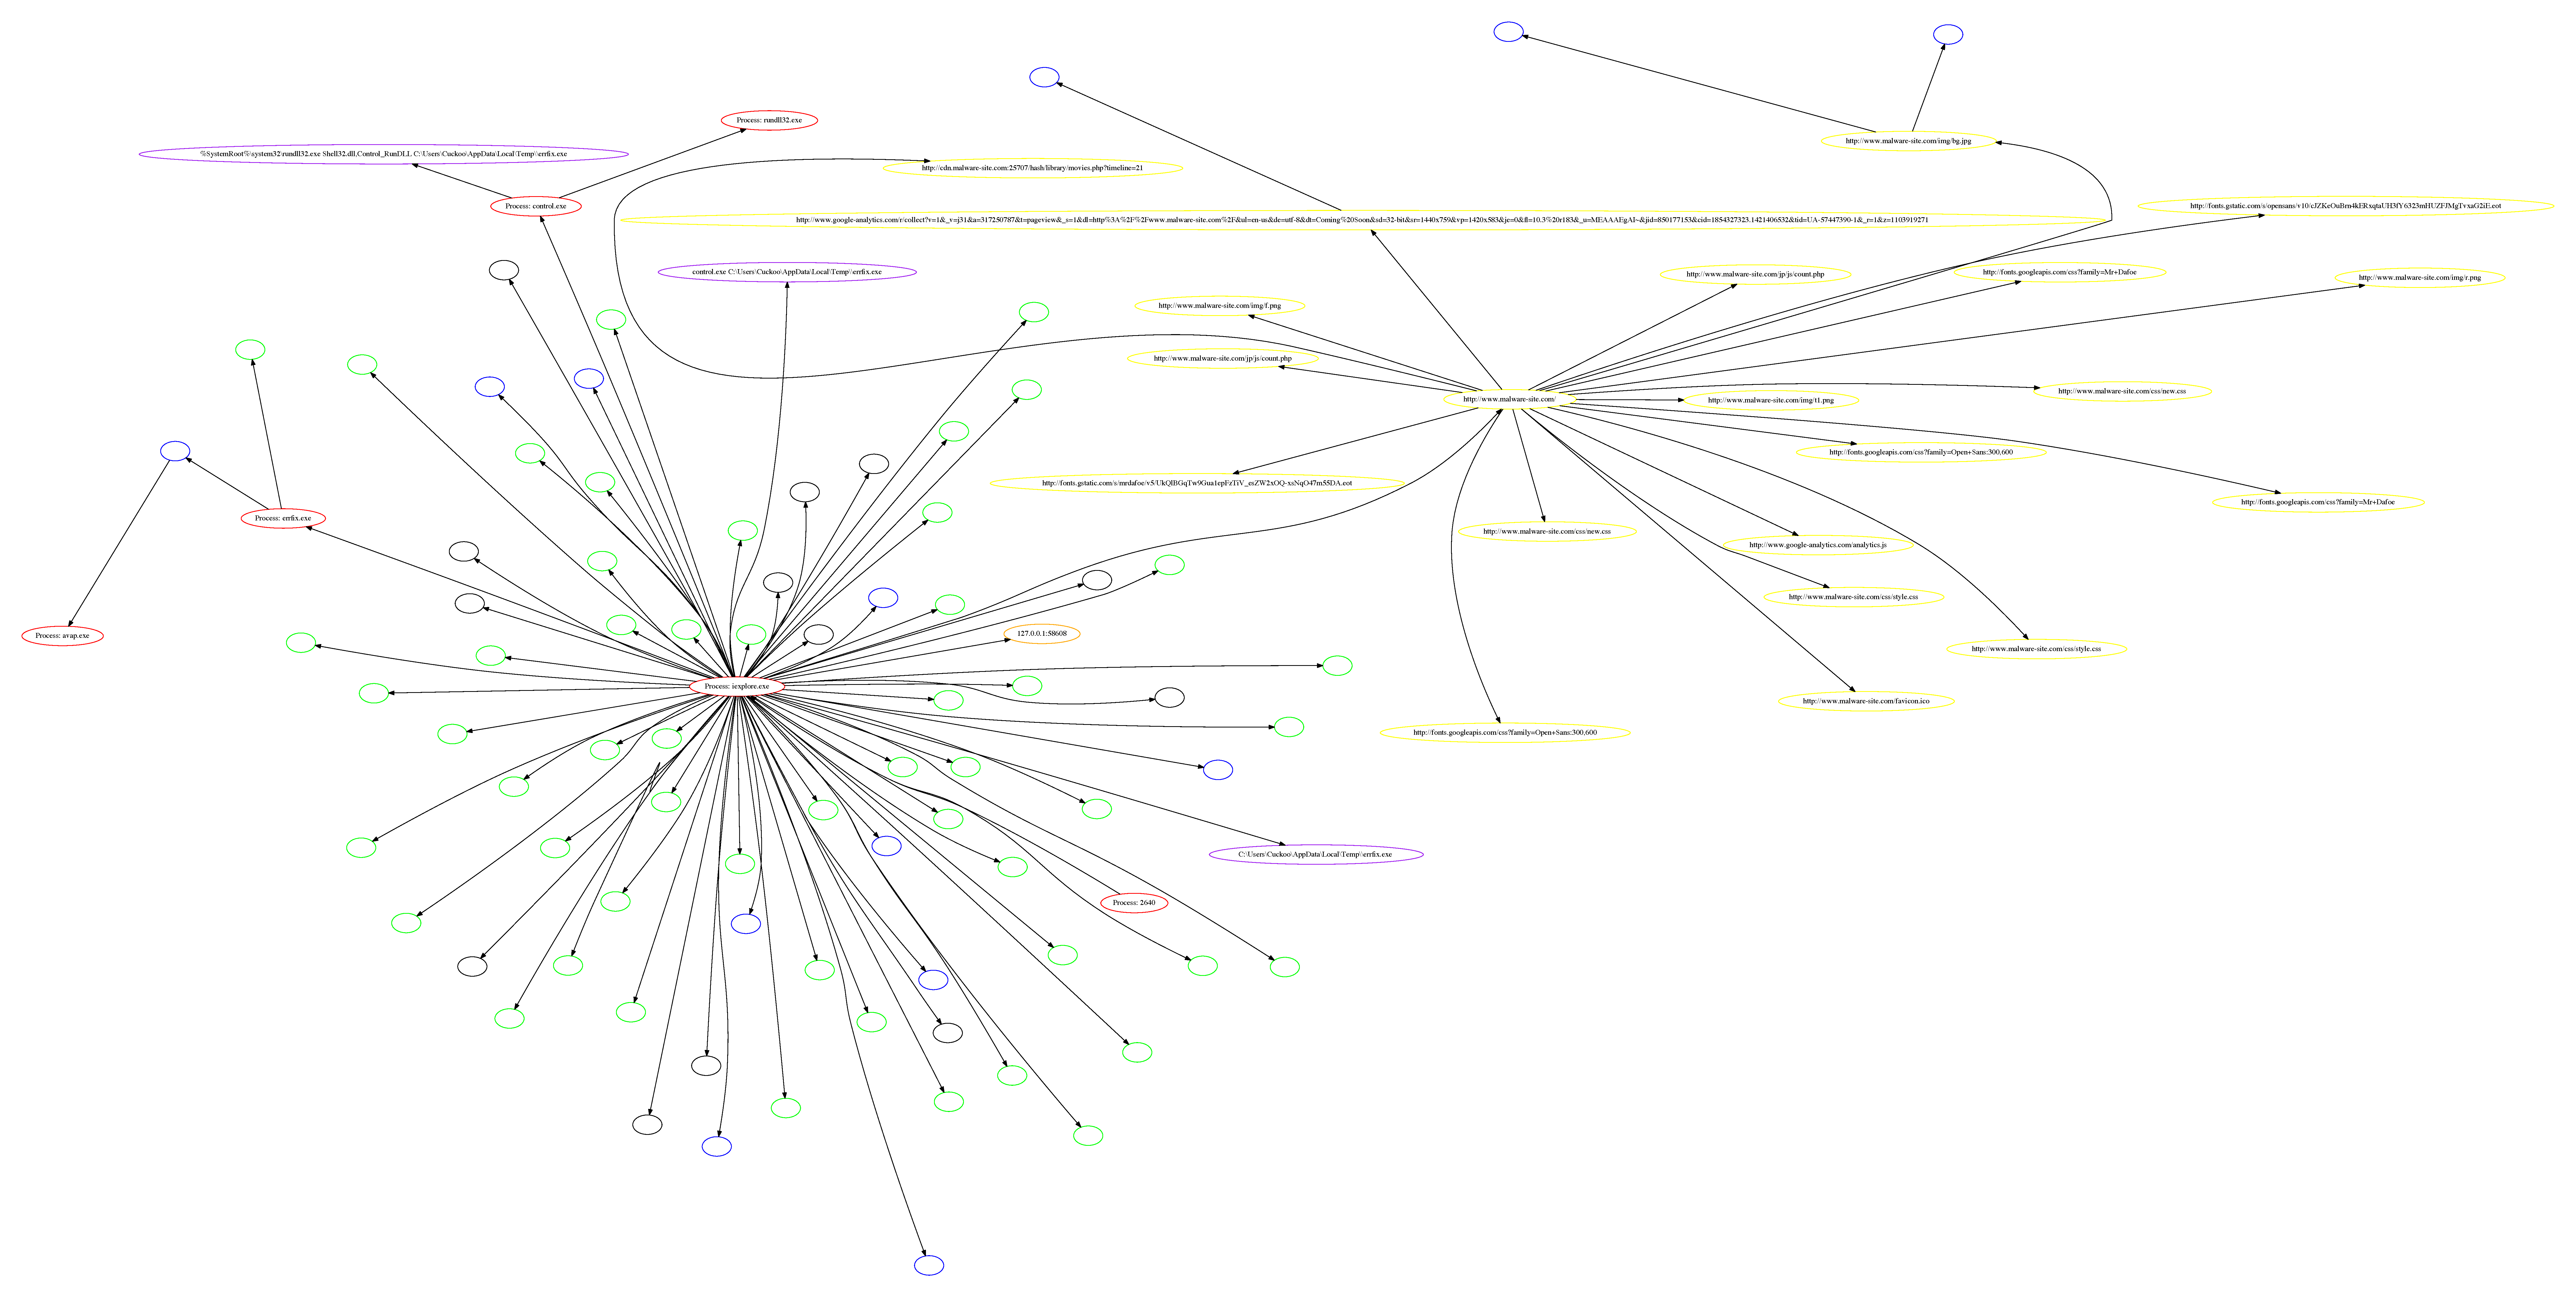
\includegraphics[width=25cm, angle=90]{Images/report_Subprocess_from_tab}
    \caption{An example of the subgraph of a single website that injected the virtual machine with malware. For clarity are only the labels of the nodes of visited URLs, involved processes and executed shell commands showed.}
    \label{fig:subgraph}
\end{figure}

\restoregeometry
\todo{Speedboost tussen Cuckoo 1.2-dev en onze wijzigingen in grafiekje zetten}



\clearpage

\section{Conclusion}
%How can we concurrently visit multiple URLs and still be able to determine which URL was responsible for malicious activities?

%\item Which techniques are used by browsers to make concurrently visiting multiple URLs possible?
%\item Which APIs are used by web browsers to make HTTP requests and retrieve webpages?
%\item How can we link an HTTP request to its source URL without the modification of the used web browser?
%\item What extra information from the client's (running) machine can be used to augment the information gained from network traffic to make the tracking of malware to its source URL easier?

In this research project was focussed on the question how the detection of drive-by download infections of malware can be improved by the means of concurrently visiting multiple URLs and still be able to determine which URL was responsible for malicious activities. To reach this goal four sub-questions have been formulated that have been answered.

Browsers implement the ability to concurrently visit multiple URLs all in a different way. Some browsers decided to use multiple threads in a single process, but most modern browsers use subprocesses dedicated to a single or a few URLs. When multiple processes are used, it depends on the implementation if that process is directly fetching the webpages or that the main process or an intermediate process is used.

How webpages are retrieved and the involved APIs highly depend on the implementation. Two of the examined browsers use the high-level HTTP library provided by the operating system while others implement their own. Such implementations are, for example, a custom library that is independent from other components of the web browser and an implementation where the network library is tightly integrated in the browser engine.

By monitoring the API calls to the network stack and the process and thread context they are made from, an individual HTTP request can be linked to where it originates from. While other methods are possible, this way no modifications to the web browser are required while still all information is available.

Additional information that can be used to detect the malicious behaviour includes process, file, registry and other network related API calls. While information sources like network sniffing, syscall observation and other passive techniques could be used, no additional information would be gained.

Based on this research, this paper proposes an algorithm that enables the possibility to do large-scale drive-by download detection by concurrently visiting multiple URLs and still be able to determine the responsible URL for the observed malicious behaviour. To validate the working and effectiveness of this algorithm, a proof of concept has been developped for an existing solution for the detection of drive-by downloads. A performance gain of xx\todo{} percent has been observed.

\clearpage

\section{Future work}
- analyser op de DAG?

\clearpage

\section*{Acknowledgements}
\addcontentsline{toc}{section}{Acknowledgements}

We would like to thank our supervisors, Jop van der Lelie and Wouter Katz from the Dutch National Cyber Security Center, for the support and insight they have given during our research project. They have greatly improved the quality of this paper.

We would also like to thank the Cuckoo developers (especially Jurriaan Bremer) who helped us understand the inner workings of Cuckoo and even helped us resolving the bugs we introduced during this project.

\clearpage

\addcontentsline{toc}{section}{References}
\bibliographystyle{abbrv}
\bibliography{report}

\clearpage

\section*{Appendix A: Simple Analyser}
\addcontentsline{toc}{section}{Appendix A: Simple Analyser}

To implement step 3 of the algorithm a very simple analyser was written which detects a process spawn beneath tab processes. Although the real code\footnote{\url{https://github.com/MartijnB/cuckoo/blob/multi-url/utils/mass-analyse.py}} is a bit unclear, it is the same as the pseudo code in listing \ref{analysercode}.

\begin{lstlisting}[caption={Pseudo code for phase 3 of the algorithm},label={analysercode}]
function deep_process_spawn_analyser(graph)
    foreach vertex in graph
        if vertex.type == "process_spawned"
            if check_depth_in_graph(vertex, 0) > 1
                print "Malicious activity"
            endif
        endif
    endforeach
endfunction

function check_depth_in_graph(vertex, current_depth)
    parents = get_parents_of_vertex(vertex)
    # Actually we need only one parent
    if length_array(parents) > 0
        return check_depth_in_graph(parents[0], current_depth++)
    else
        # No more parents, we're at the root node
        return current_depth
    endif
endfunction
\end{lstlisting}

\clearpage

\section*{Appendix B: Raw benchmark data}
\addcontentsline{toc}{section}{Appendix B: Raw benchmark data}

Table \ref{rawdata} shows the raw values (in seconds) as gathered during the benchmarks. Every value equals to a single run. The first two columns show the existing malware detection systems: Anubis and Cuckoo. The other columns show the data of the proof of concept developed for this project. The URLs used for this benchmark are random selected from the top 100 of a worldwide list\footnote{http://www.alexa.com/topsites} with the most populair websites.

\begin{table}[h]
\center
\begin{tabular}{@{}llllllll@{}}
\toprule
1 URL       & 5 URLs      & 10 URLs    \\ \midrule
\multicolumn{1}{r}{260s} & \multicolumn{1}{r}{1463s} & \multicolumn{1}{r}{2810s} \\
\multicolumn{1}{r}{311s} & \multicolumn{1}{r}{1296s} & \multicolumn{1}{r}{2702s} \\
\multicolumn{1}{r}{267s} & \multicolumn{1}{r}{1526s} & \multicolumn{1}{r}{2749s} \\
\multicolumn{1}{r}{299s} & \multicolumn{1}{r}{1373s} & \multicolumn{1}{r}{2923s} \\
\multicolumn{1}{r}{283s} & \multicolumn{1}{r}{1387s} & \multicolumn{1}{r}{2779s} \\
\multicolumn{1}{r}{271s} & \multicolumn{1}{r}{1318s} & \\
\multicolumn{1}{r}{270s} & \multicolumn{1}{r}{1353s} & \\
\multicolumn{1}{r}{250s} & \multicolumn{1}{r}{1390s} & \\
\multicolumn{1}{r}{282s} & \multicolumn{1}{r}{1448s} & \\
\multicolumn{1}{r}{265s} & \multicolumn{1}{r}{1417s} & \\
\multicolumn{1}{r}{251s} &  & \\
\multicolumn{1}{r}{264s} &  & \\
\multicolumn{1}{r}{264s} &  & \\
\multicolumn{1}{r}{279s} &  & \\
\multicolumn{1}{r}{255s} &  & \\
\multicolumn{1}{r}{357s} &  & \\
\multicolumn{1}{r}{251s} &  & \\
\multicolumn{1}{r}{279s} &  & \\
\multicolumn{1}{r}{275s} &  & \\
\multicolumn{1}{r}{265s} &  & \\
\multicolumn{1}{r}{298s} &  & \\
\multicolumn{1}{r}{256s} &  & \\
\multicolumn{1}{r}{256s} &  & \\
\multicolumn{1}{r}{271s} &  & \\
\multicolumn{1}{r}{277s} &  & \\ \bottomrule
\end{tabular}
\caption{Raw values of the benchmarks of Anubis in seconds.}
\label{rawdata_an}
\end{table}

\begin{table}[h]
\center
\begin{tabular}{@{}llllllll@{}}
\toprule
1 URL       & 5 URLs      & 10 URLs      & 25 URLs      \\ \midrule
\multicolumn{1}{r}{148,5s} & \multicolumn{1}{r}{650,6s} & \multicolumn{1}{r}{1616,2s} & \multicolumn{1}{r}{3776,9s} \\
 \multicolumn{1}{r}{161,2s} & \multicolumn{1}{r}{764,0s} & \multicolumn{1}{r}{1541,5s} & \multicolumn{1}{r}{3971,7s} \\
 \multicolumn{1}{r}{152,2s} & \multicolumn{1}{r}{736,8s} & \multicolumn{1}{r}{1519,0s} & \multicolumn{1}{r}{3812,1s} \\
 \multicolumn{1}{r}{152,1s} & \multicolumn{1}{r}{771,2s} & \multicolumn{1}{r}{1462,0s} & \multicolumn{1}{r}{3799,3s} \\
 \multicolumn{1}{r}{143,4s} & \multicolumn{1}{r}{749,0s} & \multicolumn{1}{r}{1504,7s} & \multicolumn{1}{r}{3752,4s} \\
 \multicolumn{1}{r}{149,5s} & \multicolumn{1}{r}{723,8s} & \multicolumn{1}{r}{1600,0s} & \multicolumn{1}{r}{4762,5s} \\
 \multicolumn{1}{r}{152,9s} & \multicolumn{1}{r}{971,5s} & \multicolumn{1}{r}{1530,7s} & \multicolumn{1}{r}{3968,9s} \\
 \multicolumn{1}{r}{146,0s} & \multicolumn{1}{r}{738,8s} & \multicolumn{1}{r}{1520,9s} & \multicolumn{1}{r}{3990,1s} \\
 \multicolumn{1}{r}{159,0s} & \multicolumn{1}{r}{748,6s} & \multicolumn{1}{r}{1539,2s} & \multicolumn{1}{r}{4042,0s} \\
 \multicolumn{1}{r}{148,3s} & \multicolumn{1}{r}{742,3s} & \multicolumn{1}{r}{1532,4s} & \multicolumn{1}{r}{4030,6s} \\
 \multicolumn{1}{r}{153,5s} & \multicolumn{1}{r}{754,2s} & \multicolumn{1}{r}{1414,6s} & \multicolumn{1}{r}{3899,7s} \\
 \multicolumn{1}{r}{147,9s} & \multicolumn{1}{r}{771,5s} & \multicolumn{1}{r}{1825,4s} & \multicolumn{1}{r}{3878,4s} \\
 \multicolumn{1}{r}{160,7s} & \multicolumn{1}{r}{1013,1s} & \multicolumn{1}{r}{1702,2s} & \multicolumn{1}{r}{3735,5s} \\
 \multicolumn{1}{r}{152,3s} & \multicolumn{1}{r}{728,0s} & \multicolumn{1}{r}{1458,6s} & \multicolumn{1}{r}{4023,4s} \\
 \multicolumn{1}{r}{144,0s} & \multicolumn{1}{r}{648,7s} & \multicolumn{1}{r}{1539,1s} & \multicolumn{1}{r}{3845,5s} \\
 \multicolumn{1}{r}{146,8s} & \multicolumn{1}{r}{712,1s} & \multicolumn{1}{r}{1618,3s} & \multicolumn{1}{r}{3853,7s} \\
 \multicolumn{1}{r}{164,3s} & \multicolumn{1}{r}{738,2s} & \multicolumn{1}{r}{1504,3s} & \multicolumn{1}{r}{3777,3s} \\
 \multicolumn{1}{r}{148,6s} & \multicolumn{1}{r}{785,5s} & \multicolumn{1}{r}{1488,2s} & \multicolumn{1}{r}{3923,2s} \\
 \multicolumn{1}{r}{152,5s} & \multicolumn{1}{r}{850,2s} & \multicolumn{1}{r}{1485,1s} & \multicolumn{1}{r}{4021,3s} \\
 \multicolumn{1}{r}{146,2s} & \multicolumn{1}{r}{910,1s} & \multicolumn{1}{r}{1504,3s} & \multicolumn{1}{r}{3921,2s} \\
 \multicolumn{1}{r}{148,1s} & \multicolumn{1}{r}{728,8s} & \multicolumn{1}{r}{1804,9s} & \multicolumn{1}{r}{3792,8s} \\
 \multicolumn{1}{r}{185,5s} & \multicolumn{1}{r}{751,5s} & \multicolumn{1}{r}{1786,5s} & \multicolumn{1}{r}{3990,1s} \\
 \multicolumn{1}{r}{161,1s} & \multicolumn{1}{r}{755,0s} & \multicolumn{1}{r}{1554,4s} & \multicolumn{1}{r}{3972,7s} \\
 \multicolumn{1}{r}{144,1s} & \multicolumn{1}{r}{751,7s} & \multicolumn{1}{r}{1548,9s} & \multicolumn{1}{r}{4154,6s} \\
 \multicolumn{1}{r}{151,9s} & \multicolumn{1}{r}{746,2s} & \multicolumn{1}{r}{1779,8s} & 3982,2 \\ \bottomrule
\end{tabular}
\caption{Raw values of the benchmarks of Cuckoo in seconds.}
\label{rawdata_cuckoo}
\end{table}

\begin{table}[h]
\center
\begin{tabular}{@{}llllllll@{}}
\toprule
1 URL       & 5 URLs      & 10 URLs      & 25 URLs      & 50 URLs      & 100 URLs     \\ \midrule
\multicolumn{1}{r}{44,8s}       & \multicolumn{1}{r}{93,7s}       & \multicolumn{1}{r}{109,3s}       & \multicolumn{1}{r}{144,2s}       & \multicolumn{1}{r}{271,0s}       & \multicolumn{1}{r}{455,9s}        \\
\multicolumn{1}{r}{45,2s}       & \multicolumn{1}{r}{85,3s}       & \multicolumn{1}{r}{100,4s}       & \multicolumn{1}{r}{140,5s}       & \multicolumn{1}{r}{240,3s}       & \multicolumn{1}{r}{431,9s}        \\
\multicolumn{1}{r}{45,2s}       & \multicolumn{1}{r}{67,7s}       & \multicolumn{1}{r}{84,0s}        & \multicolumn{1}{r}{152,2s}       & \multicolumn{1}{r}{251,8s}       & \multicolumn{1}{r}{438,8s}        \\
\multicolumn{1}{r}{47,1s}       & \multicolumn{1}{r}{59,9s}       & \multicolumn{1}{r}{86,9s}        & \multicolumn{1}{r}{146,0s}       & \multicolumn{1}{r}{272,2s}       & \multicolumn{1}{r}{456,9s}        \\
\multicolumn{1}{r}{44,9s}       & \multicolumn{1}{r}{67,6s}       & \multicolumn{1}{r}{141,0s}       & \multicolumn{1}{r}{156,4s}       & \multicolumn{1}{r}{254,7s}       & \multicolumn{1}{r}{482,3s}        \\
\multicolumn{1}{r}{43,8s}       & \multicolumn{1}{r}{83,5s}       & \multicolumn{1}{r}{100,8s}       & \multicolumn{1}{r}{155,7s}       & \multicolumn{1}{r}{252,3s}       & \multicolumn{1}{r}{414,2s}        \\
\multicolumn{1}{r}{46,2s}       & \multicolumn{1}{r}{74,8s}       & \multicolumn{1}{r}{90,0s}        & \multicolumn{1}{r}{138,4s}       & \multicolumn{1}{r}{247,9s}       & \multicolumn{1}{r}{480,1s}        \\
\multicolumn{1}{r}{44,7s}       & \multicolumn{1}{r}{65,1s}       & \multicolumn{1}{r}{135,1s}       & \multicolumn{1}{r}{153,5s}       & \multicolumn{1}{r}{240,7s}       & \multicolumn{1}{r}{430,7s}        \\
\multicolumn{1}{r}{47,8s}       & \multicolumn{1}{r}{92,5s}       & \multicolumn{1}{r}{87,2s}        & \multicolumn{1}{r}{161,5s}       & \multicolumn{1}{r}{257,5s}       & \multicolumn{1}{r}{410,6s}        \\
\multicolumn{1}{r}{60,0s}       & \multicolumn{1}{r}{63,9s}       & \multicolumn{1}{r}{93,5s}        & \multicolumn{1}{r}{172,8s}       & \multicolumn{1}{r}{297,0s}       & \multicolumn{1}{r}{429,2s}        \\
\multicolumn{1}{r}{47,0s}       & \multicolumn{1}{r}{76,4s}       & \multicolumn{1}{r}{103,4s}       & \multicolumn{1}{r}{185,4s}       & \multicolumn{1}{r}{248,3s}       & \multicolumn{1}{r}{452,5s}        \\
\multicolumn{1}{r}{47,6s}       & \multicolumn{1}{r}{106,5s}      & \multicolumn{1}{r}{90,0s}        & \multicolumn{1}{r}{144,1s}       & \multicolumn{1}{r}{265,3s}       & \multicolumn{1}{r}{442,3s}        \\
\multicolumn{1}{r}{52,5s}       & \multicolumn{1}{r}{74,4s}       & \multicolumn{1}{r}{128,0s}       & \multicolumn{1}{r}{156,0s}       & \multicolumn{1}{r}{582,7s}       & \multicolumn{1}{r}{537,1s}        \\
\multicolumn{1}{r}{51,3s}       & \multicolumn{1}{r}{64,8s}       & \multicolumn{1}{r}{95,7s}        & \multicolumn{1}{r}{156,8s}       & \multicolumn{1}{r}{265,4s}       & \multicolumn{1}{r}{461,4s}        \\
\multicolumn{1}{r}{61,7s}       & \multicolumn{1}{r}{65,9s}       & \multicolumn{1}{r}{84,2s}        & \multicolumn{1}{r}{160,3s}       & \multicolumn{1}{r}{251,6s}       & \multicolumn{1}{r}{441,2s}        \\
\multicolumn{1}{r}{45,8s}       & \multicolumn{1}{r}{104,3s}      & \multicolumn{1}{r}{109,1s}       & \multicolumn{1}{r}{163,9s}       & \multicolumn{1}{r}{261,5s}       & \multicolumn{1}{r}{436,1s}        \\
\multicolumn{1}{r}{46,2s}       & \multicolumn{1}{r}{69,7s}       & \multicolumn{1}{r}{86,4s}        & \multicolumn{1}{r}{166,9s}       & \multicolumn{1}{r}{253,3s}       & \multicolumn{1}{r}{438,3s}        \\
\multicolumn{1}{r}{46,9s}       & \multicolumn{1}{r}{68,1s}       & \multicolumn{1}{r}{103,5s}       & \multicolumn{1}{r}{145,9s}       & \multicolumn{1}{r}{332,1s}       & \multicolumn{1}{r}{465,9s}        \\
\multicolumn{1}{r}{48,3s}       & \multicolumn{1}{r}{69,6s}       & \multicolumn{1}{r}{88,0s}        & \multicolumn{1}{r}{185,9s}       & \multicolumn{1}{r}{535,8s}       & \multicolumn{1}{r}{409,4s}        \\
\multicolumn{1}{r}{61,2s}       & \multicolumn{1}{r}{65,5s}       & \multicolumn{1}{r}{93,3s}        & \multicolumn{1}{r}{175,4s}       & \multicolumn{1}{r}{258,9s}       & \multicolumn{1}{r}{463,5s}        \\
\multicolumn{1}{r}{54,1s}       & \multicolumn{1}{r}{70,6s}       & \multicolumn{1}{r}{138,8s}       & \multicolumn{1}{r}{202,8s}       & \multicolumn{1}{r}{259,4s}       & \multicolumn{1}{r}{466,5s}        \\
\multicolumn{1}{r}{45,7s}       & \multicolumn{1}{r}{67,0s}       & \multicolumn{1}{r}{104,7s}       & \multicolumn{1}{r}{186,5s}       & \multicolumn{1}{r}{284,9s}       & \multicolumn{1}{r}{481,0s}        \\
\multicolumn{1}{r}{42,7s}       & \multicolumn{1}{r}{74,4s}       & \multicolumn{1}{r}{110,8s}       & \multicolumn{1}{r}{165,1s}       & \multicolumn{1}{r}{260,2s}       & \multicolumn{1}{r}{451,8s}        \\
\multicolumn{1}{r}{54,1s}       & \multicolumn{1}{r}{70,4s}       & \multicolumn{1}{r}{95,8s}        & \multicolumn{1}{r}{139,7s}       & \multicolumn{1}{r}{267,6s}       & \multicolumn{1}{r}{446,4s}        \\
\multicolumn{1}{r}{45,9s}       & \multicolumn{1}{r}{69,5s}       & \multicolumn{1}{r}{99,8s}        & \multicolumn{1}{r}{146,3s}       & \multicolumn{1}{r}{247,6s}       & \multicolumn{1}{r}{448,0s}        \\ \bottomrule
\end{tabular}
\caption{Raw values of the benchmarks of Roadrunner in seconds.}
\label{rawdata}
\end{table}

\clearpage

\section*{Appendix C: Cuckoomon modifications}
\addcontentsline{toc}{section}{Appendix C: Cuckoomon modifications}
\label{cuckoomonmods}

Cuckoomon is the analyser component of Cuckoo. It hooks interesting API functions and logs their usage. As part of the development of the proof of concept, many hooks have been disabled and several missing ones added.

\textbf{Added hooks}

\begin{longtable}{*{2}{>{\arraybackslash}p{6cm}}}
URLDownloadToFileA     & HttpSendRequestExW           \\
FtpOpenFileA           & HttpEndRequestA              \\
FtpOpenFileW           & HttpEndRequestW              \\
FtpGetFileA            & HttpQueryInfoA               \\
FtpGetFileW            & HttpQueryInfoW               \\
FtpPutFileA            & InternetConfirmZoneCrossingA \\
FtpPutFileW            & InternetConfirmZoneCrossingW \\
HttpAddRequestHeadersA & InternetReadFileExA          \\
HttpAddRequestHeadersW & InternetReadFileExW          \\
HttpSendRequestExA     &                             
\end{longtable}

\textbf{Removed hooks}

\begin{longtable}{*{2}{>{\arraybackslash}p{6cm}}}
NtReadFile            & NtDeviceIoControlFile   \\
NtQueryDirectoryFile  & NtQueryInformationFile  \\
NtOpenDirectoryObject & FindFirstFileExA        \\
FindFirstFileExW      & GetDiskFreeSpaceExA     \\
GetDiskFreeSpaceExW   & GetDiskFreeSpaceA       \\
GetDiskFreeSpaceW     & RegEnumKeyW             \\
RegEnumKeyExA         & RegEnumKeyExW           \\
RegEnumValueA         & RegEnumValueW           \\
RegQueryValueExA      & RegQueryValueExW        \\
RegQueryInfoKeyA      & RegQueryInfoKeyW        \\
NtEnumerateKey        & NtEnumerateValueKey     \\
NtQueryValueKey       & NtQueryMultipleValueKey \\
NtLoadKey             & NtLoadKey2              \\
NtLoadKeyEx           & NtQueryKey              \\
FindWindowA           & FindWindowW             \\
FindWindowExA         & FindWindowExW           \\
EnumWindows           & NtOpenMutant            \\
NtOpenSection         & ZwMapViewOfSection      \\
ExitProcess           & NtUnmapViewOfSection    \\
NtFreeVirtualMemory   & SetWindowsHookExA       \\
SetWindowsHookExW     & UnhookWindowsHookEx     \\
LdrGetDllHandle       & LdrGetProcedureAddress  \\
ExitWindowsEx         & LookupPrivilegeValueW   \\
WriteConsoleA         & WriteConsoleW           \\
GetSystemMetrics      & GetCursorPos            \\
GetComputerNameA      & GetComputerNameW        \\
GetUserNameA          & GetUserNameW            \\
NtDelayExecution      & GetLocalTime            \\
GetSystemTime         & GetTickCount            \\
NtQuerySystemTime     & send                    \\
sendto                & recv                    \\
recvfrom              & select                  \\
connect               & WSARecv                 \\
WSARecvFrom           & WSASend                 \\
WSASendTo             & CryptProtectData        \\
CryptUnprotectData    & CryptProtectMemory      \\
CryptUnprotectMemory  & CryptDecrypt            \\
CryptEncrypt          & CryptHashData           \\
CryptDecodeMessage    & CryptDecryptMessage     \\
CryptEncryptMessage   & CryptHashMessage       
\end{longtable}

\end{document}
